\documentclass{article}
\headheight=8pt \topmargin=10pt
\textheight=624pt \textwidth=432pt
\oddsidemargin=18pt \evensidemargin=18pt

\usepackage{epsfig,amsfonts,latexsym,amsmath,amssymb,mathtools}
\usepackage{caption,footmisc}
\usepackage{authblk}

\usepackage[latin1]{inputenc}
%\usepackage{tikz}
%\usetikzlibrary{arrows,shapes,positioning,shadows,trees,decorations.shapes}
%\usetikzlibrary{decorations.text}

\renewcommand{\thefootnote}{\fnsymbol{footnote}}
%\renewcommand*{\thefootnote}{\arabic{footnote}}
%\renewcommand{\thefootnote}{\ifcase\value{footnote}\or(*)\or
%	(**)\or(***)\or(****)\or(\#)\or(\#\#)\or(\#\#\#)\or(\#\#\#\#)\or($\infty$)\fi}

\newcommand{\dd}{\mathrm{d}}

\graphicspath{{../figs/}}

\title{ESCI520 course project: Machine learning for earthquake detection}
\author{Katherine Begland}
\author{John Cornthwaite}
\author{Xiaobo Meng}
\author{Jia Shi}
\author{Neng Xiong}
\affil{Department of Earth, Environmental and Planetary Sciences, Rice University.}

\begin{document}
%\pagestyle{empty}

	\maketitle    
	 % intro
\section{Introduction}
The report studies and replicates elements of the FAST algorithm \cite{yoon2015earthquake}. 
     % data processing
\section{Data processing}

     % template
\section{Template matching}
we use templates with high SNR to cross-correlate with the continuous data to detect other events. The Figure \ref{fig:method} shows one example of this method.
\begin{figure}[htbp] 
\centering 
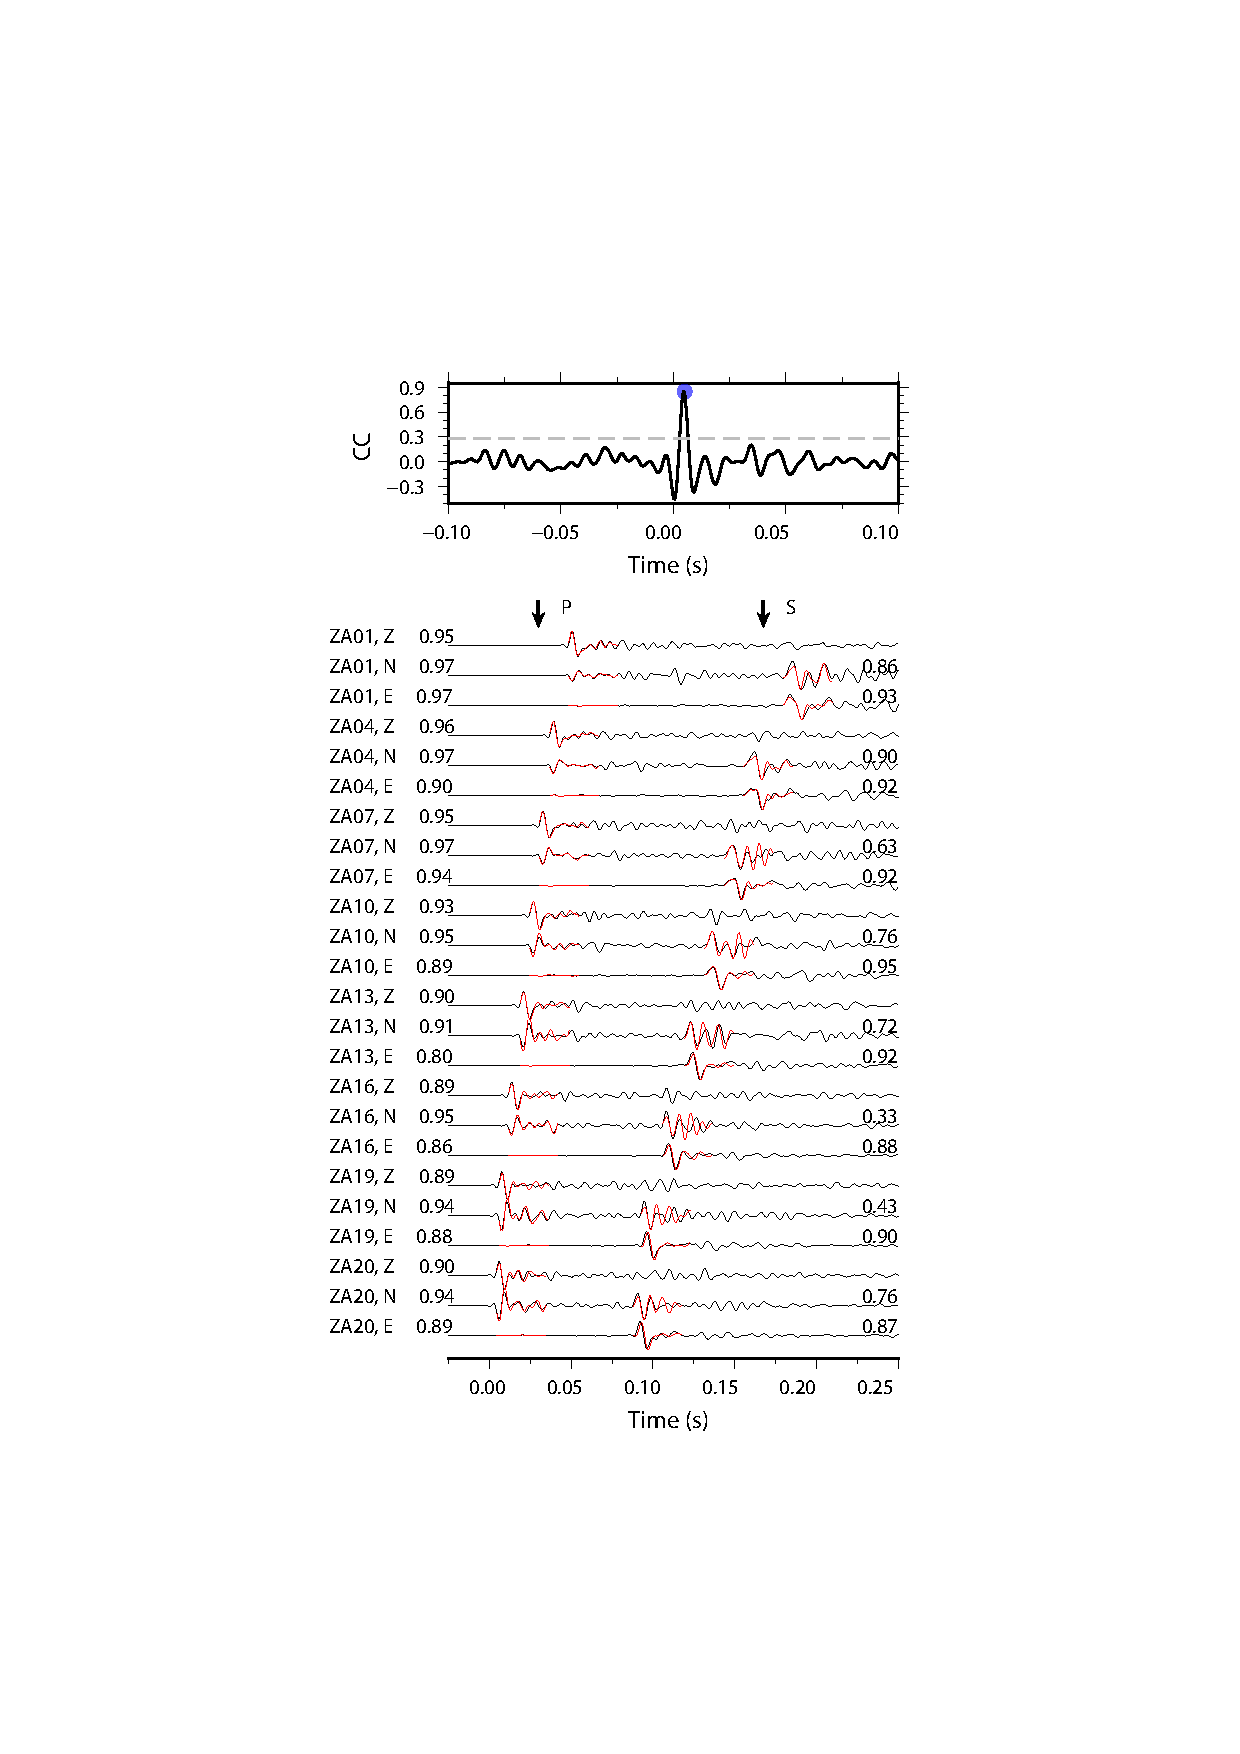
\includegraphics[height=6cm, width=3cm]{Template-search} 
\caption{\label{fig:method} (a) Stacked cross-correlograms. (b) Waveform comparison between the master event (red) and the target slave event (black) for the three components of several selected receiver levels.} 
\end{figure}
  In this project, we use 14 templates and detect 22 events. Among the 22 events, there are 8 events can obviously observed.


    
    \bibliographystyle{plain}
    \bibliography{ESCI520FAST}
% bib
\end{document}
